%!TEX root = ../main.tex
 
\subsection{Compiling JaVerT Specifications to Symbolic Tests} 
\label{specs:example}

\myparagraph{\javert Specifications} 
\javert specifications of JavaScript functions are analogous to \jsil specifications of \jsil procedures, and are of the form $\specsig{P_{\jssuffix}}{\fid(\jvec{x})}{Q_{\jssuffix}}{\flag}$. A~\javert specification $\specsig{P_{\jssuffix}}{\fid(\jvec{x})}{Q_{\jssuffix}}{\flag}$
is valid for a JavaScript program $\jstmt$, written $\jstmt \satisfies \specsig{P_{\jssuffix}}{\fid(\jvec{x})}{Q_{\jssuffix}}{\flag}$, 
if and only if $\jstmt$ contains a function literal with identifier $\fid$ and ``whenever $\fid$ is executed in a state satisfying $P_\jssuffix$, then, 
if it terminates, it does so in a state satisfying $Q_\jssuffix$, with return mode $\flag$''. The assertion language used by \javert is very similar to the assertion language of \jsil Logic and is described in detail in~\cite{javert}.
There, the authors present 
a compiler from \javert specifications to \jsil Logic specifications, denoted by $\ltr$, and prove the soundness 
of that compiler, assuming a correct compiler $\compile$ from JavaScript to~\jsil.
This theoretical result ensures that the verification of \jsil programs can be lifted to   the verification of JavaScript programs. More concretely, a \javert  specification $\specsig{P_{\jssuffix}}{\fid(\jvec{x})}{Q_{\jssuffix}}{\flag}$
is valid for a given JavaScript program $\jstmt$ if and only if the translated specification 
$\ltr(\specsig{P_{\jssuffix}}{\fid(\jvec{x})}{Q_{\jssuffix}}{\flag})$ is valid for the compilation 
of $\jstmt$ by a correct compiler $\compile$. Put formally:  
\begin{equation}
   \jstmt \vDash  \specsig{P_{\jssuffix}}{\fid(\jvec{x})}{Q_{\jssuffix}}{\flag} 
      \iff
           \compile(\jstmt) \vDash \ltr(\specsig{P_{\jssuffix}}{\fid(\jvec{x})}{Q_{\jssuffix}}{\flag}).
\end{equation}

We generate symbolic tests from JavaScript programs and their \javert specifications in the following way. First, we convert the JavaScript program and its \javert specification to a \jsil program with its \jsil Logic specification, using the \JSComp and $\ltr$ compilers. Next, we 
generate a set of symbolic tests from the obtained \jsil program and \jsil Logic specification, as described in \S\ref{specs:to:symbolic:tests}. 
Finally, we run the generated \jsil symbolic tests on the \jsil symbolic execution engine. If \jilette finds a bug while running these tests, we will obtain a concrete counter-example triggering that bug.

\begin{figure}[t!]
\centering
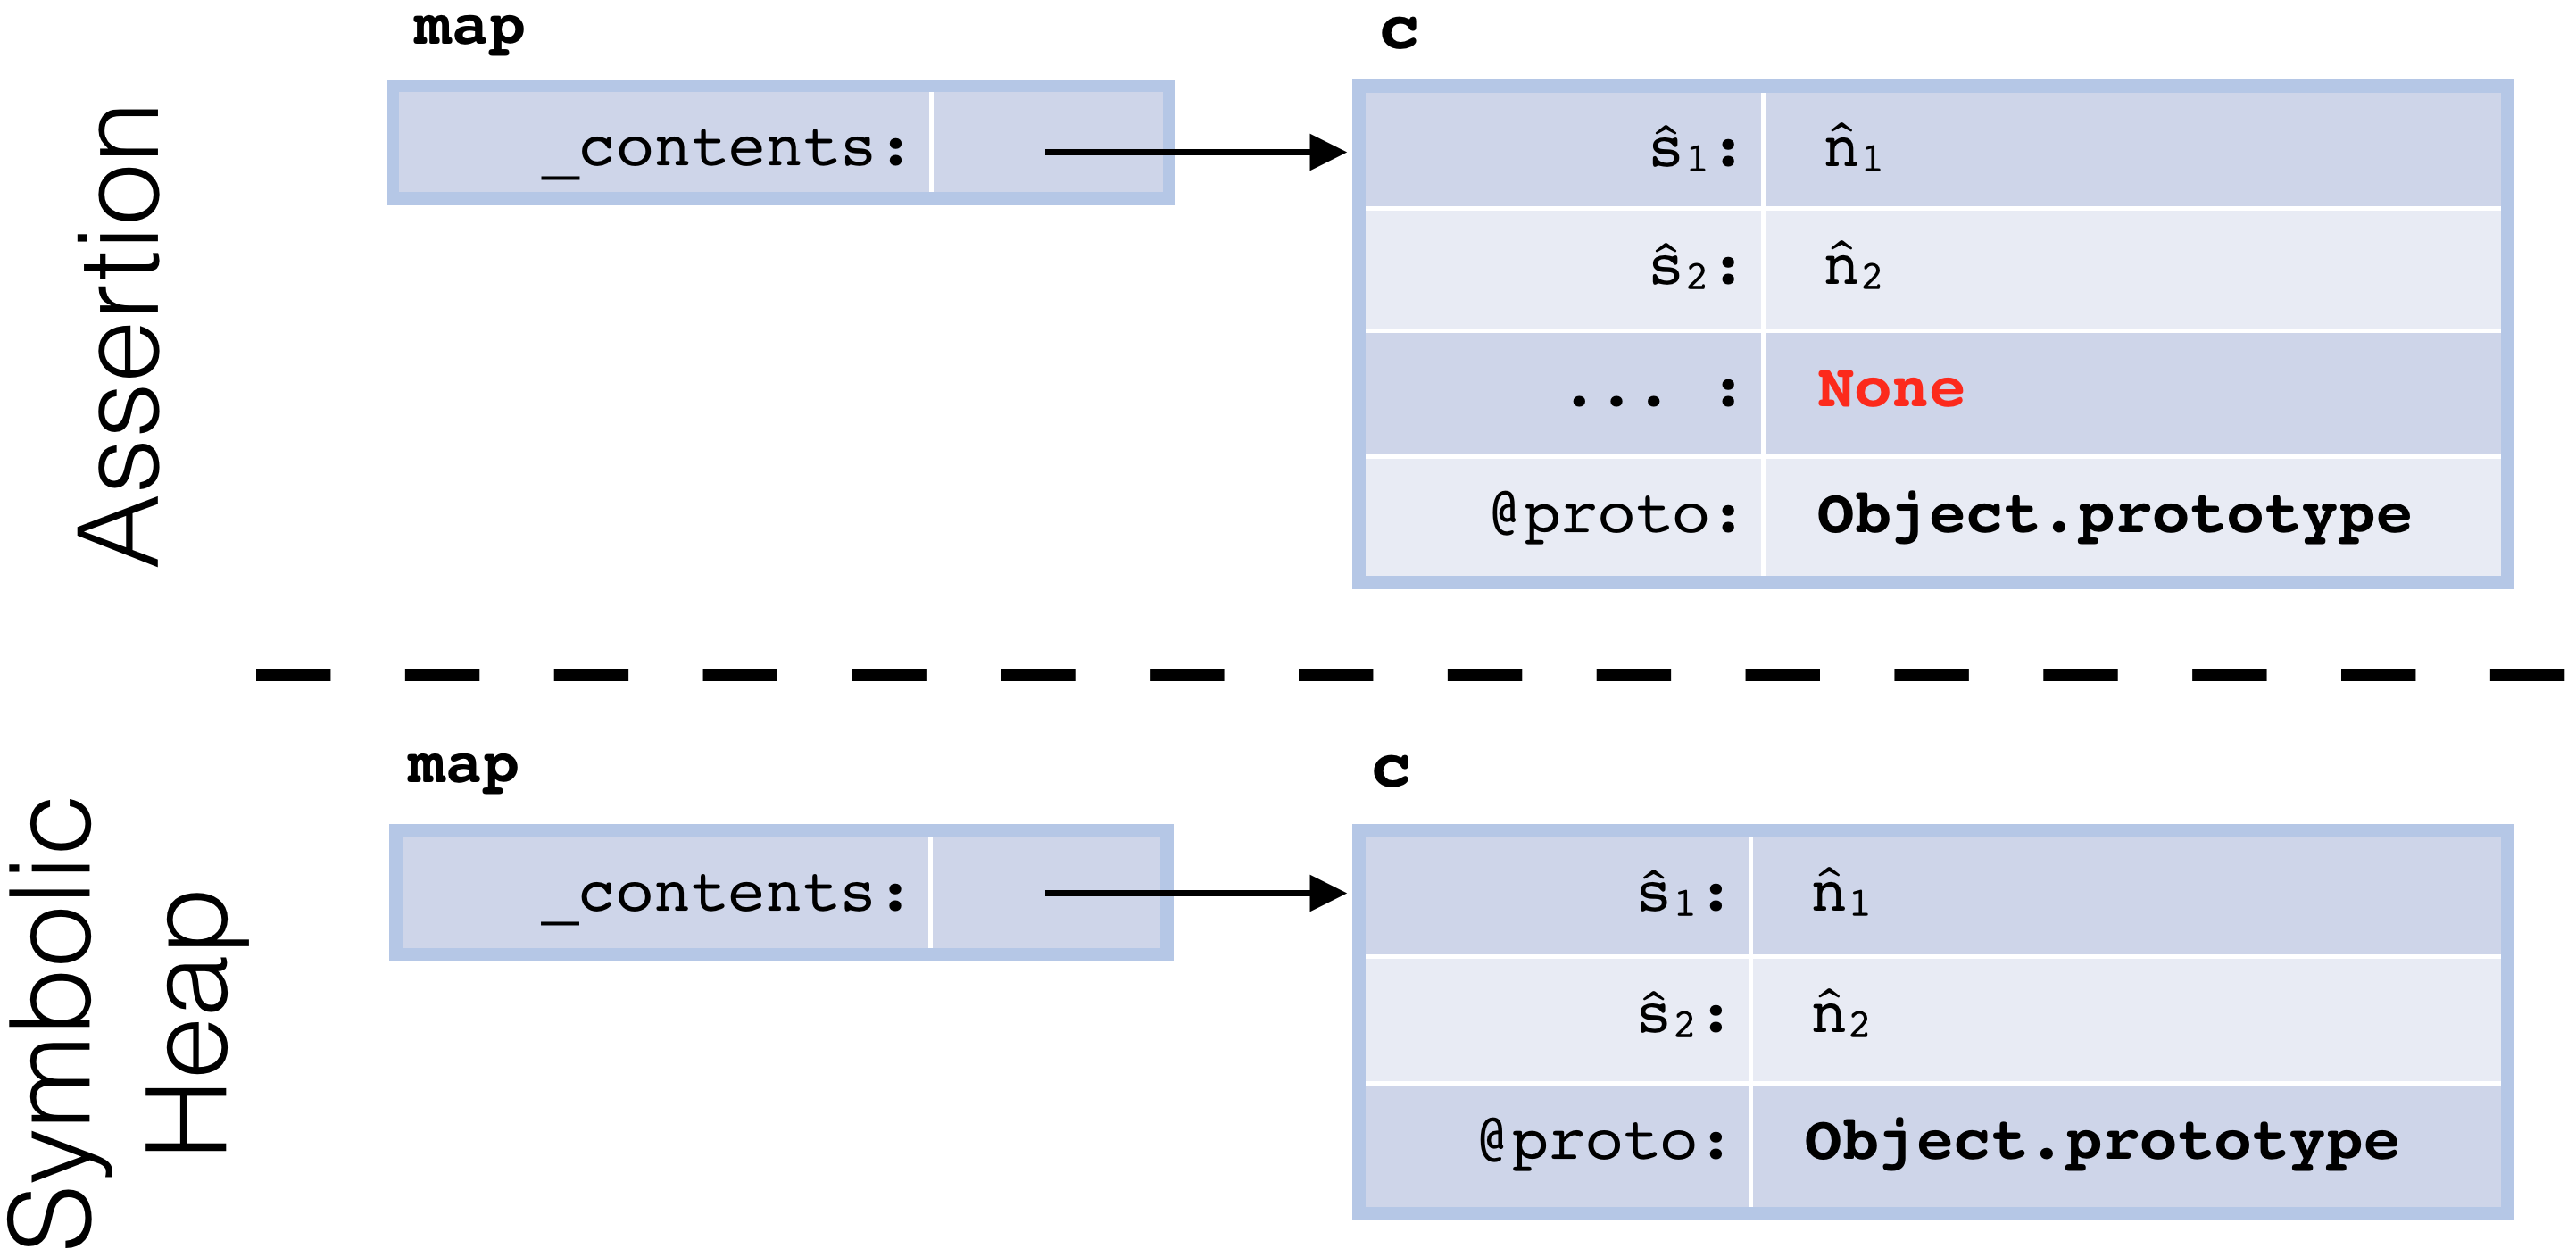
\includegraphics[width=\linewidth]{figures/symbvsass.png}

\vspace*{-0.7cm}
{\small $$
\text{\emph{Negative resource constraints: }} \{ \hat{s}_1, \hat{s}_2 \} \subseteq \{ \hat{s}_1, \hat{s}_2 \}
$$}
\vspace{-0.8cm}
\caption{Assertion vs. Symbolic Heap: {\small$\mathtt{Map(map, \{ (\hat{s}_1, \hat{n}_1), (\hat{s}_2, \hat{n}_2) \} )}$}}\label{fig:symb:state:versus:assertion}
\vspace{-0.5cm}
\end{figure}

\myparagraph{Example}
We illustrate the debugging of SL-specifications by appealing to the \jsinline|Map| example shown in Figure \ref{map:example}. In order to reason about a key-value map,
we define several predicates, whose definitions we show below.

\begin{Verbatim}[fontsize=\footnotesize,commandchars=\\\{\}]
Map (m, kvs) := 
  DataProp(m, "_contents", c) * JSObject(c) * 
    KVPairs(c, kvs) * first(kvs, keys) * emptyFields(c, keys)
\end{Verbatim}
 \begin{Verbatim}[fontsize=\footnotesize,commandchars=\\\{\}]
KVPairs (o, kvs) := 
  (kvs = \{ \}),
  (kvs = (k, v) -u- kvs') * ValidKey(k) * DataProp(o, k, v) * KVPairs(o, kvs')
\end{Verbatim}
\begin{Verbatim}[fontsize=\footnotesize,commandchars=\\\{\}]
ValidKey (k) := types(k : Str) * \textcolor{red}{(k <> "hasOwnProperty")}
\end{Verbatim}

The \jsinline|Map| predicate captures the resource corresponding to a map object. 
Concretely, it first states that the map object has the property \jsinline|_contents|, which points to a default JavaScript object \jsinline|c|, using the predicates \jsinline|DataProp| and \jsinline|JSObject|. 
\jsinline|DataProp(o, p, v)| captures the property \jsinline|p| of object \jsinline|o| and states that it has value \jsinline|v|, while abstracting over other associated JavaScript internals, whereas \jsinline|JSObject(o)| states that the object \jsinline|o| is an extensible object of class \jsinline|"Object"|, whose prototype is \jsinline|Object.prototype| (for more details, see~\cite{javert}). 
Next, using the \jsinline|KVPairs| predicate (explained shortly), it states that \jsinline|c| holds the key-value pairs \jsinline|kvs|. Finally, it states that \jsinline|c| has no other properties except the keys present in \jsinline|kvs|. For this, it first obtains the set of keys from the set of key-value pairs \jsinline|kvs| using the predicate \jsinline|first(kvs, keys)|, which states that the first projection of \jsinline|kvs| equals \jsinline|keys| (its definition is standard), and then uses the \jsinline|emptyFields| assertion to state that all other properties are absent from the object.

The \jsinline|KVPairs(o, kvs)| predicate talks about key-value pairs of an object \jsinline|o|. 
It is defined recursively on the structure of \jsinline|kvs| and it has two definitions, separated by a comma. 
We have that \jsinline|kvs| is either empty or that it contains at least one key-value pair \jsinline|(k, v)|.\footnote{We write {\small\texttt{-u-}} for set union and omit the brackets around singleton sets.} 
In the latter case, we state that the key \jsinline|k| must be valid, that the object \jsinline|o| has the property \jsinline|k| with value \jsinline|v|, and proceed recursively.
Note that the uniqueness of keys in \jsinline|kvs| is guaranteed by the \jsinline|DataProp| predicate of \jsinline|KVPairs| and the separating conjunction.

The \jsinline|ValidKey(k)| predicate captures the validity of a given key and holds \emph{iff} the corresponding JavaScript function \jsinline|validKey(k)| returns \jsinline|true|.
In the definition of \jsinline|ValidKey|, we highlight in red a potential source of errors on which we will focus shortly.

To give a better intuition of how the \jsinline|Map| predicate works, we show the full unfolding of {\small$\mathtt{Map(map, \{ (\hat{s}_1, \hat{n}_1), (\hat{s}_2, \hat{n}_2) \} )}$} in Figure \ref{fig:symb:state:versus:assertion}.
%a \emph{map object predicate}, \jsinline|Map|, 
%which uses the auxiliary predicate \jsinline|KVPairs|, capturing the resource of the key-value pairs in the map, 
%and the \jsinline|validKey(k)| predicate, which captures the validity of a key and holds if and only if the corresponding JavaScript function \jsinline|ValidKey(k)| returns \jsinline|true|\footnote{For the moment, we treat the $\mathtt{ValidKey}$ predicate as a black box.}.
%
%Intuitively, the \jsinline|Map(m, kvs)| predicate captures the resource 
%of a map object \jsinline|m| with key-value pairs \jsinline|kvs| (a set of string-number pairs, modelled as two-element lists).
%%\footnote{We model pairs as lists with two elements and, for clarity, use the pair notation.}). 
%For instance, the assertion $\mathtt{Map(map, \{ (\hat{s}_1, \hat{n}_1), (\hat{s}_2, \hat{n}_2) \} )}$ can be unfolded as illustrated in Figure~\ref{fig:symb:state:versus:assertion}. 
%Observe that the definition of \jsinline|Map| does not include the resource of a map prototype, as it is shared between all map objects, and therefore needs to be factored out.  
%
There, we can also see how the negative resource captured by the SL-assertion {\small$\mathtt{Map(map, \{ (\hat{s}_1, \hat{n}_1), (\hat{s}_2, \hat{n}_2) \} )}$}, namely the resource captured by {\small$\mathtt{emptyFields(c, first(kvs))}$}, disappears from the symbolic heap and is transformed into the negative resource constraint $\{ \hat{s}_1, \hat{s}_2 \} \subseteq \{ \hat{s}_1, \hat{s}_2 \}$, which states that all properties of the object \jsinline|c| in the symbolic heap (in our case, $\hat{s}_1$ and $\hat{s}_2$) must be in the set of properties of the corresponding \jsinline|emptyFields| assertion (in our case, {\small$\mathtt{first(\{ (\hat{s}_1, \hat{n}_1), (\hat{s}_2, \hat{n}_2) \}) = \{ \hat{s}_1, \hat{s}_2 \}}$}).
Such constraints are generated in item ${\bf e.}$ of the test generation algorithm presented in Figure \ref{fig:test:generation}. 

Below, we show the relevant parts of the specifications of \jsinline|get(k)| and \jsinline|put(k, v)|, for the case in which
 \jsinline|k| already exists in the map:

\noindent
\begin{minipage}{\linewidth}
\begin{displaymath} 
{\scriptsize
\hspace*{-0.2cm}
\begin{array}{c}
\left\{ {\begin{array}{c}
 \text{\texttt{Map(this, kvs -u- (k, v)) * ObjProtoF() *}} \\
 \text{\texttt{(this, "@proto") -> mp * MapProto(mp) * ...}}
\end{array}} \right\} \\
%
\text{\bfseries \texttt{get(k)}} \\[0.2mm]
%
\left\{ {\begin{array}{c}
 \text{\texttt{Precondition * (ret = v)}} 
\end{array}} \right\}
\end{array}
} 
\end{displaymath}
\end{minipage}
\quad
\begin{minipage}{\linewidth}
%
\begin{displaymath} 
{\scriptsize
\begin{array}{c}
\left\{ {\begin{array}{c}
 \text{\texttt{Map(this, kvs -u- (k, v')) * ObjProtoF() *}} \\
 \text{\texttt{(this, "@proto") -> mp * MapProto(mp) * ...}}
\end{array}} \right\} \\
%
\text{\bfseries \texttt{put(k, v)}} \\[0.2mm]
%
\left\{ {\begin{array}{c}
 \text{\texttt{Map(this, kvs -u- (k, v)) * ObjProtoF() *}} \\
 \text{\texttt{(this, "@proto") -> mp * MapProto(mp) * ...}}
\end{array}} \right\}
\end{array}
} 
\end{displaymath}
\end{minipage}

\vspace{10pt}
The predicate \jsinline|ObjProtoF()| describes the resource captured by the \jsinline|Object.prototype| object. 
In particular, it is needed because \texttt{get} uses the \texttt{hasOwnProperty} function, which is defined as a property of \jsinline|Object.prototype|. 
The predicate \jsinline|MapProto| specifies the resource of a valid map prototype: in particular, the map prototype needs to define the methods \jsinline|put|, \jsinline|get|, and \jsinline|validKey|. Finally, note that, given the definition of the \jsinline|Map| and \jsinline|KVPairs| predicates, both preconditions shown entail that \jsinline|k| is a valid key.

\begin{figure}[t!]
\centering
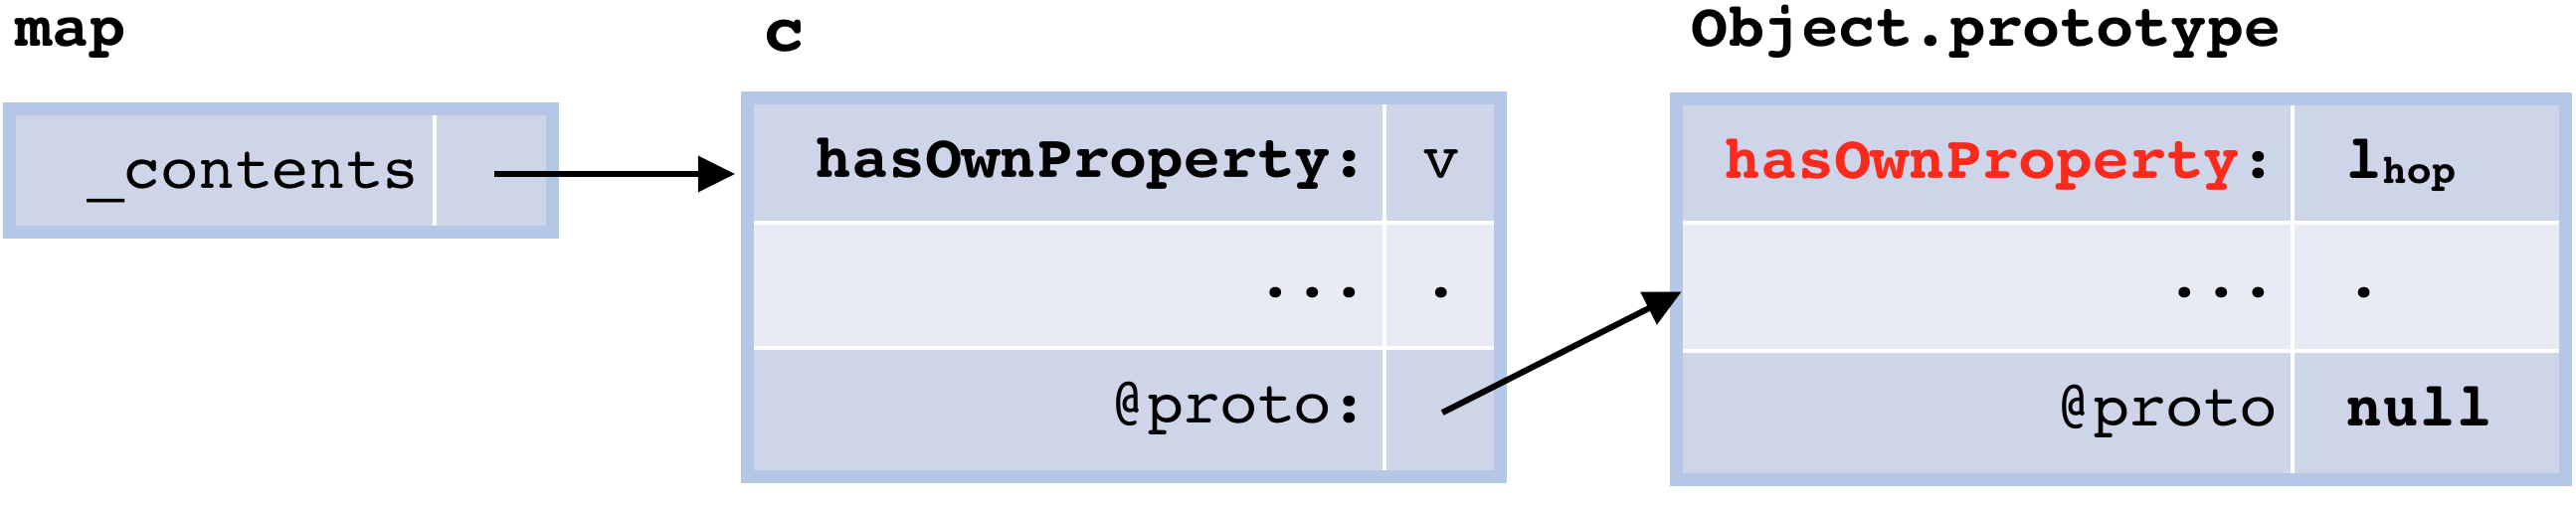
\includegraphics[width=\linewidth]{figures/heapfail.png}
\caption{Property shadowing: \jsinline|c.hasOwnProperty(...)| cannot reach \jsinline|Object.prototype|.} 
\label{fig:cexget}
\vspace{-0.5cm}
\end{figure}

Now, if we forgot to state the part of the $\mathtt{ValidKey(k)}$ predicate highlighted in red, that is, if we did not state that $\mathtt{k}$ needed to be different from \jsinline|"hasOwnProperty"|, the symbolic test generated for the specification of \jsinline|get| would fail for unfoldings of $\mathtt{KVPairs}$ of depth $\geq 1$, with the counter-model \jsinline|k = "hasOwnProperty"|. 
In that case, as illustrated in Figure~\ref{fig:cexget}, the \jsinline|"hasOwnProperty"| property of \jsinline|Object.prototype| would no longer be reachable by property lookup from \jsinline|c|, and
the execution of line~5 (\jsinline|if (c.hasOwnProperty(k))|) would raise an error, as it would attempt to call the \jsinline|"hasOwnProperty"| property of object \jsinline|c| as a function instead. 
Since this specification of $\mathtt{get(k)}$ requires normal termination, the jump to the error label in the compiled \jsil code will trigger the $\assert(\jfalse)$ of the generated symbolic test and the developer will be presented with the counter-model \jsinline|k = "hasOwnProperty"|.

\begin{center}
\polish{What else would we like to say here?}
\end{center}
